\begin{tabularx}{\linewidth}{|X|X|X|X|}
    \hline
    \textbf{Sin} & \textbf{Cos} & \textbf{Tan} & \textbf{Cot}\\
    \hline
    \textbf{G} & \textbf{A} & \textbf{G} & \textbf{A}\\
    \hline
    \textbf{H} & \textbf{H} & \textbf{A} & \textbf{G}\\
    \hline
\end{tabularx}

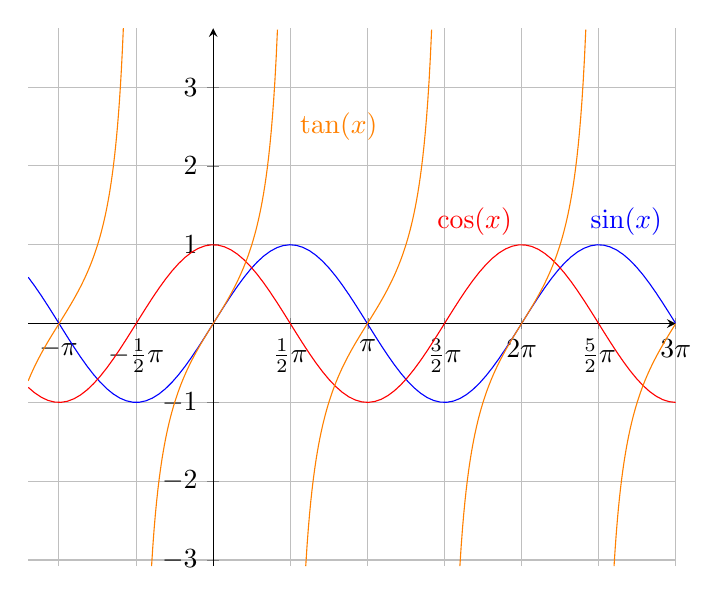
\begin{tikzpicture}
\begin{axis}[enlargelimits=false,
             axis lines=middle,
             scale=1.2,
             xtick={-3.15159, -1.57080, 0,
                     1.57080,  3.15159, 4.71239,
                     6.28318,  7.85398, 9.42478 }, 
             xticklabels={$-\pi$, $-\frac{1}{2}\pi$, 0,
                          $\frac{1}{2}\pi$, $\pi$, $\frac{3}{2}\pi$,
                          $2\pi$, $\frac{5}{2}\pi$, $3\pi$ },
             ytick={-3,-2,-1,0,1,2,3},
             grid=major, % only a grid on the defined ticks
             samples=100 % number of points
             ]
 
  % sin
  \addplot[blue,no marks,domain=-1.2*pi:3*pi]{sin(deg(x))}; % deg to convert radians
  \node[right=10pt,above] at (axis cs:5*pi/2,1){\color{blue}$\sin(x)$};
 
  % cos
  \addplot[red,no marks,domain=-1.2*pi:3*pi] {cos(deg(x))};
  \node[above left] at (axis cs:2*pi,1){\color{red}$\cos(x)$};
 
  % tan, multiple parts because of singularities
  \addplot[orange,no marks,domain=-1.2*pi:-0.583*pi, ]{tan(deg(x))};
  \addplot[orange,no marks,domain=-0.4*pi:5*pi/12,   ]{tan(deg(x))};
  \addplot[orange,no marks,domain=27*pi/45:17*pi/12, ]{tan(deg(x))};
  \addplot[orange,no marks,domain=1.6*pi:29*pi/12,   ]{tan(deg(x))};
  \addplot[orange,no marks,domain=2.6*pi:36*pi/12,   ]{tan(deg(x))};
  \node[right] at (axis cs:pi/2,2.5){\color{orange}$\tan(x)$};
 
\end{axis}
\end{tikzpicture}